\newpage
	\section{C} \label{sec:C}

		\subsection{CAMMINO CRITICO} \index{Cammino critico} \label{camminocritico}
		Sequenza di attività ordinata con prodotto importante e dipendenze temporali strette. Miro al cammino di peso massimo.

		\subsection{CAPABILITY}	\index{Capability} \label{capability} %(slide 14) Set Lezione del 4/12 - Qualità di processo
		Traduzione: possibilità/capacità. \\
		Misura l’adeguatezza di un processo per gli scopi a esso assegnati. È una caratteristica propria del processo e  determina il risultato (in termini di efficienza ed efficacia) raggiungibile per quel processo. Conviene che il livello di capability sia alto, ovvero seguito da tutti in modo disciplinato, sistematico e quantificabile.

		\subsection{CAPITOLATO D'APPALTO} \index{Capitolati d'appalto} \label{capitolati}
		Documento tecnico che descrive in maniera dettagliata tutti i bisogni. In esso vengono spiegate le cose che chi commissiona vuole, nel gergo di una persona normale. Sono interamente responsabilità del cliente e da esso ne conseguono:
			\begin{itemize}
				\item \textbf{Requisiti utente} che sono vincoli contrattuali che specificano il \textit{cosa}
				\item \textbf{Requisiti software} che specificano il \textit{come}
			\end{itemize}

		\subsection{CICLO DI DEMING} \index{Ciclo di Deming} \label{pdca}
		Il ciclo di Deming (o ciclo di PDCA) è un metodo di gestione iterativo per il controllo e il miglioramento continuo dei processi e dei prodotti, suddiviso in 4 fasi:
			\begin{itemize}
				\item \textbf{\underline{\hyperref[pianificazione]{Plan}}}: definisce attività, scadenze, ecc. necessari a raggiungere specifici obiettivi di miglioramento
				\item \textbf{Do}: esegue le attività di \textit{Plan}
				\item \textbf{Check}: verifica l'esito delle azione di miglioramento rispetto alle attese
				\item \textbf{Act}: consolida il tutto e cerca dei modi per il miglioramento successivo
			\end{itemize}

		\subsection{CICLO DI VITA} \index{Ciclo di vita} \label{ciclo}
		Si riferisce alla completa durata del prodotto, dal concepimento al ritiro (= fine) che deve essere garantita. È da vedersi come una macchina a \underline{\hyperref[stato]{stati}} in cui ho una certa sequenza di passaggi da seguire. La transizione tra stati avviene tramite l’esecuzione di
		attività di processi di ciclo di vita. Lo stazionamento in uno stato o transizione viene detta \underline{\hyperref[fase]{fase}}. In seguito al ritiro, il prodotto può essere ``rimesso in vita'', per questo viene chiamato \textit{ciclo}.

		\begin{figure}[H]
			\centering
			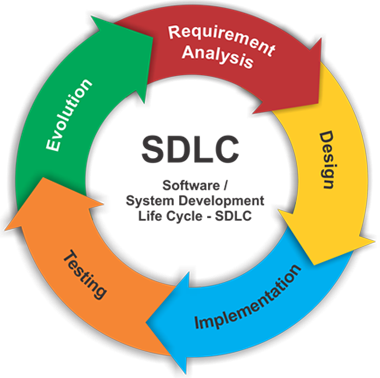
\includegraphics[width=0.5\textwidth]{img/lifecycle}
			\caption{I 5 stati del ciclo di vita di un prodotto.}
		\end{figure}

		Associare un sistema di \underline{\hyperref[qualita]{qualità}} al modello adottato, aiuta a perseguire conformità nel \underline{\hyperref[progetto]{progetto}} e \underline{\hyperref[maturita]{maturità}} nei processi.	Conoscere il ciclo di vita previsto di un prodotto, aiuta a valutarne preventivamente i tempi, i costi e i rischi. \\
		Esistono:
		\begin{itemize}
			\item \underline{\hyperref[processo]{Processi}} di ciclo di vita, che specificano le \textit{attività} da svolgere per abilitare le transizioni di stato nel ciclo di vita
			\item \underline{\hyperref[modelli]{Modelli}} di ciclo di vita, che descrivono questi processi e come concorrono ad abilitare le specifiche transizioni
		\end{itemize}
		Per organizzare le attività dei processi implicati, è necessario identificare le dipendenze tra gli ingressi dell'uno e le uscite dell'altro, in modo da fissare quindi l'ordinamento nel tempo e i criteri di attivazione e completamento.

		\subsection{CLASSIFICAZIONE DEI REQUISITI} \index{Classificazione dei requisiti} \label{classificazione}
		Guardo in generale i \underline{\hyperref[requirements]{requisiti}} e li classifico in base a:
		\begin{itemize}
			\item \textbf{Cosa devo fare} con il prodotto, quindi secondo gli attributi del prodotto (ho dei requisiti funzionali)
			\item \textbf{Come devo farlo}, quindi secondo i processi (ho dei requisiti di vincolo)
		\end{itemize}

		\subsection{CMMI}	\index{CMMI} \label{cmmi} %(slide 11) Set Lezione del 4/12 - Qualità di processo
		CMM (\textit{\underline{\hyperref[capability]{Capability}} \underline{\hyperref[maturita]{Maturity}} Model}) evoluto poi in CMMI (\textit{Capability Maturity Model Integration}) è un \textit{modello di valutazione} (\underline{\hyperref[standard]{standard}}) uniforme dei fornitori. \\
		\textit{Model} è l'insieme di criteri per valutare il grado di \underline{\hyperref[qualita]{qualità}} (in scala assoluta) dei processi dell’azienda, mentre \textit{Integration} è l'architettura di integrazione delle diverse discipline (system, HW, SW) e tipologie di attività delle aziende.

		\subsection{CoCoMo}	\index{CoCoMo} \label{cocomo}
		\textit{Constructive Cost Model} è un modello algoritmico che stima le risorse necessarie esprimendone la misura in mesi/persona (\texttt{MP}). 1MP sono 152 ore. \\
		Questo modello è da utilizzare per la \underline{\hyperref[gestioneprogetto]{gestione di progetto}}.
		%[Per formule e il resto vedi slide 21/35-24/35]

		\subsection{COESO} \index{Coeso} \label{coeso}
		Ciò che è coeso indica avere delle attività messe insieme a un dato scopo, che devono esserci e se non ci fossero se ne sentirebbe la mancanza.  \\
		Per quel che riguarda le componenti di un'\underline{\hyperref[architettura]{architettura}} possiamo dire che funzionalità ``vicine'' devono stare nella stessa componente e dato che la modularità spinge a decomporre il grande in piccolo, la ricerca di coesione fornisce un criterio di decomposizione. \par
		La coesione \emph{va massimizzata} per ottenere maggiore manutenibilità e riusabilità, minor legame fra componenti e maggiore comprensibilità dell’architettura del sistema. La coesione inoltre si può misurare. \\
		Ci sono diversi tipi di buona coesione (la migliore è sempre quella che persegue \textit{information hiding}):
			\begin{itemize}
				\item \textbf{Funzionale}: quando le parti concorrono allo stesso specifico compito.
				\item \textbf{Sequenziale}: quando alcune azioni sono più ``vicine'' ad altre per ordine di esecuzione ed è conveniente tenerle insieme.
				\item \textbf{Informativa}: quando le parti agiscono sulla stessa unità d'informazione
				(la \underline{\hyperref[best]{best practice}}).
			\end{itemize}

		\subsection{COLLAUDO}	\index{Collaudo}	\label{collaudo}
		È l'atto formale di verifica di efficienza o di validità.  Ad esso segue il rilascio del prodotto e la fine della commessa.

		\subsection{COMMITTENTE} \index{Committente} \label{committente}
		Persona che ha il compito di identificare il prodotto da commissionare.

		\subsection{COMPONENTE} \index{Componente} \label{componente}
		Radice della composizione, ovvero non soltanto è una parte, ma è fatto per essere messo insieme ad altre parti.

		\subsection{COMPORTAMENTO PREDICIBILE}	\label{comportamentopredicibile} %13 dicembre - verifica e validazione: analisi statica
		Ci interessa garantire comportamento predicibile del software, ovvero che ``lo posso dire prima'', perché non ci sia ambiguità. Gli \textit{elementi di vulnerabilità} per garantire comportamento predicibile del SW sono:
		\begin{itemize}
			\item \textbf{Effetti laterali} (side-effect): la causa sono variabili condivise. La soluzione è l'\underline{\hyperref[incapsulamento]{incapsulamento}}.
			\item \textbf{Ordine}: di due importanti momenti:
			\begin{itemize}
				\item \textbf{Elaborazione}, ovvero preparare le risorse logiche di cui il programma avrà bisogno al principio, ad esempio avere un po' di RAM, quindi preparare l'ambiente di esecuzione
				\item \textbf{Inizializzazione}, ovvero dichiarare le variabili prima di fare \textit{begin}
			\end{itemize}
			\item \textbf{Passaggio di parametro}: per valore e per riferimento (ricordo che in Java le variabili vengono passate ad una funzione facendone una copia e ricordare esempio dello swap che non fa effettivamente lo scambio). %slide 8/30
		\end{itemize}


		\subsection{COMPUTATIONAL THINKING} \index{Computational thinking} \label{computational}
		L'insieme dei processi mentali coinvolti nella formulazione di un problema e della sua soluzione, in modo tale che un umano o una macchina possa effettivamente eseguirlo. La cosa giusta da fare è aumentare abilità e sfide proporzionalmente.


		\subsection{CONFIGURAZIONE} \index{Configurazione} \label{configurazione}
		Indica le parti di un prodotto software e come esse vengono messe insieme.


		\subsection{CONSIDERAZIONI PRAGMATICHE} \index{Considerazioni pragramtiche}	\label{pragmatico}
		%slide 11/30 di Lez17: Verifica e validazione - Analisi statica
		Termine legato a \underline{\hyperref[programmiverificabili]{programmi verificabili}}. \\
		L’efficacia dei metodi di verifica è funzione della qualità di strutturazione del codice. Ad esempio una procedura con un solo punto di ingresso e un solo punto di uscita è più facilmente analizzabile per il suo effetto sullo stato. \\
		La verifica di un programma relaziona frammenti di codice con frammenti di specifica: la verificabilità è funzione inversa dell’ampiezza del contesto. Conviene quindi confinare gli ambiti e la visibilità.


		\subsection{CONSUNTIVO} \index{Consuntivo} \label{consuntivo}
		Rendiconto dei risultati di un dato periodo di attività di un ente o di un'impresa, che si stima verso la fine.
		Esistono:
			\begin{itemize}
				\item \textbf{Consuntivo di periodo}: ogni azione in questo periodo chiede nuova pianificazione sul rimanente (il prodotto è la pianificazione del residuo)
				\item \textbf{\underline{\hyperref[preventivo]{Preventivo}} a finire}: conseguente al consuntivo di periodo
			\end{itemize}


		\subsection{CONTROLLO} \index{Controllo} \label{controllo}
			\subsubsection{Di Versione}  \label{controllodiversione} \index{Controllo di versione}
			Riguarda la gestione della storia di un prodotto.
			\subsubsection{Di Configurazione}  \label{controllodiconfigurazione} \index{Controllo di configurazione}
			Riguarda la frammentazione del codice in parti (ad esempio perchè non vogliamo 2000 righe di codice in un file).


		\subsection{CONTROLLO DI QUALITÀ}	\index{Controllo di Qualità}	\label{controlloqualita} %slide 9/22 Set Qualità del software
		Controllo di Qualità (o \textit{Quality Assurance}) sono le attività del sistema qualità pianificate e attuate per assicurare che il prodotto soddisfi le attese. \\
		Si può fare in due modi:
		\begin{itemize}
			\item \textbf{Assaggiatore}: ogni prodotto realizzato lo faccio valutare (non è la miglior soluzione perchè non vado a monte del problema, potrei sprecare risorse)
			\item \textbf{Quality assurance}: perseguendo attivamente altrimenti è uno sforzo collettivo. Bisogna avere un \underline{\hyperref[way]{way of working}} che mostri fiducia e controllo a monte. Ma tutto questo deve avvenire in modo non invasivo. Conviene seguire uno \underline{\hyperref[standard]{standard}}.
		\end{itemize}


		\subsection{CORRETTEZZA}	\index{Correttezza} \label{correttezza}
			\subsubsection{Per costruzione}	\label{byconstruction}
			\textit{``Correctness by construction''} vuol dire avere strumenti oggettivi misurabili che ci dicono se stiamo andando bene. Con regole di questo tipo, sono confidente di quello che ho fatto.
			\subsubsection{Per correzione} \label{bycorrection}
			\textit{``Correctness by correction''} vuol dire provarci, cercando di sistemare pezzo per pezzo. Non sappiamo quindi effettivamente se funziona.


		\subsection{COVERAGE}	\index{Coverage}	\label{coverage}
		Il \textit{fattore di copertura} è quanto la prova fa esercitare il prodotto rispetto alla percentuale di:
		\begin{itemize}
			\item Funzionalità esercitate come viste dall'esterno: \textbf{copertura funzionale}
			\item Logica interna del codice esercitata: \textbf{copertura strutturale} (branch, condition)
		\end{itemize}
		\textbf{Attenzione}: una copertura al 100\% non prova assenza di difetti e in ogni caso un 100\% può essere irraggiungibile.


		\subsection{CRITERI DI PROGRAMMAZIONE}	\index{Criteri di programmazione}	\label{criteriprog}
		Criteri di programmazione: %slide 10/30 13 dicembre - verifica e validazione: analisi statica
		i \textit{criteri} (ovvero norme fondanti) servono per riconoscere i principi che ho usato per fare \underline{\hyperref[incapsulamento]{incapsulamento}} e altre norme:
		\begin{itemize}
			\item Architettura (\textit{\underline{\hyperref[progettazione]{design}}}) del codice
			\item Separazione interfaccia e implementazione: ciò rende bassissimo l'accoppiamento. L'idea è che il client non deve conoscere l'implementazione, ma solo l'interfaccia (che non deve cambiare)
			\item Massimizzazione di \textit{information hiding}
			\item Uso dei tipi (se ci sono): devo fare operazioni il cui esito sia verificabile, sapendo i tipi
		\end{itemize}


		\subsection{CUSTOMER} \index{Customer} \label{customer}
		Primo elemento di un \underline{\hyperref[progetto]{progetto}} secondo \underline{\hyperref[semat]{SEMAT}}. Comprende \underline{\hyperref[opportunity]{opportunity}} e \underline{\hyperref[stakeholder]{stakeholders}}.
